\section{Introduction}
\label{section:introduction}

\citet{Hanneke-2016} showed that for any class $C$ of Vapnik-Chervonenkis
dimension $d$ there exists an algorithm that $\epsilon$-learns any target
function from $C$ under any distribution from $O\left(\frac{d +
\log(1/\delta)}{\epsilon}\right)$ labeled examples with probability at least
$1-\delta$. For this paper, it is important to stress that Hanneke's algorithm
does \emph{not} receive the distribution of unlabeled data as input. On the
other hand, \citet{Benedek-Itai-1991} showed that for any class $C$ and any
distribution there exists an algorithm that $\epsilon$-learns any target from
$C$ from $O \left( \frac{\log N_{\epsilon/2} + \log
(1/\delta)}{\epsilon}\right)$ labeled examples with probability at least
$1-\delta$ where $N_{\epsilon/2}$ is the size of an $\frac{\epsilon}{2}$-cover
of $C$ with respect to the disagreement metric $d(f,g) = \Pr[f(x) \neq g(x)]$.
Here, it is important to note that Benedek and Itai construct for each
distribution a separate algorithm. In other words, they construct a family of
algorithms indexed by the (uncountably many) distributions over the domain.
Alternatively, we can think of Benedek-Itai's family of algorithms as a single
algorithm that receives the distribution as an input. It is known that
$N_\epsilon = O(1/\epsilon)^{O(d)}$; see \citet{Dudley-1978}. Thus, ignoring
$\log(1/\epsilon)$ factor, Benedek-Itai bound is never worse than Hanneke's
bound.

As we already mentioned, Benedek-Itai's algorithm receives as input the
distribution of unlabeled data. The algorithm uses it to construct an
$\frac{\epsilon}{2}$-cover. Unsurprisingly, there exist distributions which have
a small $\frac{\epsilon}{2}$-cover and thus sample complexity of Benedek-Itai's
algorithm on such distributions is significantly lower then the Hanneke's bound.
For instance, a distribution concentrated on a single point has an
$\frac{\epsilon}{2}$-cover of size $2$ for any positive $\epsilon$.

However, an algorithm does not need to receive the unlabeled distribution in
order to enjoy low sample complexity. For example, empirical risk minimization
(ERM) algorithm needs significantly less labeled examples to learn any target
under some unlabeled distributions. For instance, if the distribution is
concentrated on a single point, ERM needs only one labeled example to learn any
target. One could be lead to believe that there exists an algorithm that does
\emph{not} receive the unlabeled distribution as input and achieves Benedek-Itai
bound (or a slightly worse bound) for \emph{every} distribution. In fact, one
could think that ERM or Hanneke's algorithm could be such algorithms. If ERM,
Hanneke's algorithm, or some other distribution-independent algorithm had sample
complexity that matches (or nearly matches) the optimal distribution-specific
sample complexity for \emph{every} distribution, we could conclude that the
knowledge of unlabeled data distribution is completely useless.

As \citet{Darnstadt-Simon-Szorenyi-2013} showed this is not the case. They showed
that \emph{any} algorithm for learning projections over $\{0,1\}^n$ that does
not receive the unlabeled distribution as input, requires, for some data
unlabeled distributions, more labeled examples than the Benedek-Itai bound.
However, they did not quantify this gap beside stating that it grows without
bound as $n$ goes to infinity.

In this paper, we quantify the gap by showing that \emph{any}
distribution-independent algorithm for learning the class of projections over
$\{0,1\}^n$ requires, for some unlabeled distributions, $\Omega(\log n)$ times
as many labeled examples as Benedek-Itai bound.
\citet{Darnstadt-Simon-Szorenyi-2013} showed the gap for any class with
Vapnik-Chervonenkis dimension $d$ is at most $O(d)$. It is well known that
Vapnik-Chervonenkis dimensions of projections over $\{0,1\}^n$ is $\Theta(\log
n)$. Thus our lower bounds matches the upper bound $O(d)$. To better understand
the relationship of the upper and lower bounds, we illustrate the situation for
the class of projections over $\{0,1\}^n$ in
Figure~\ref{figure:sample-complexity}.

In contrast, we show that for the class of \emph{all} functions (on any domain)
there is no gap between the two settings. In other words, for learning a target
from the class of all functions, unlabeled data are in fact useless. This
illustrates the point that the gap depends in a non-trivial way on the
combinatorial structure of the function class rather than just on the
Vapnik-Chervonenkis dimension.

\begin{figure}
\centering
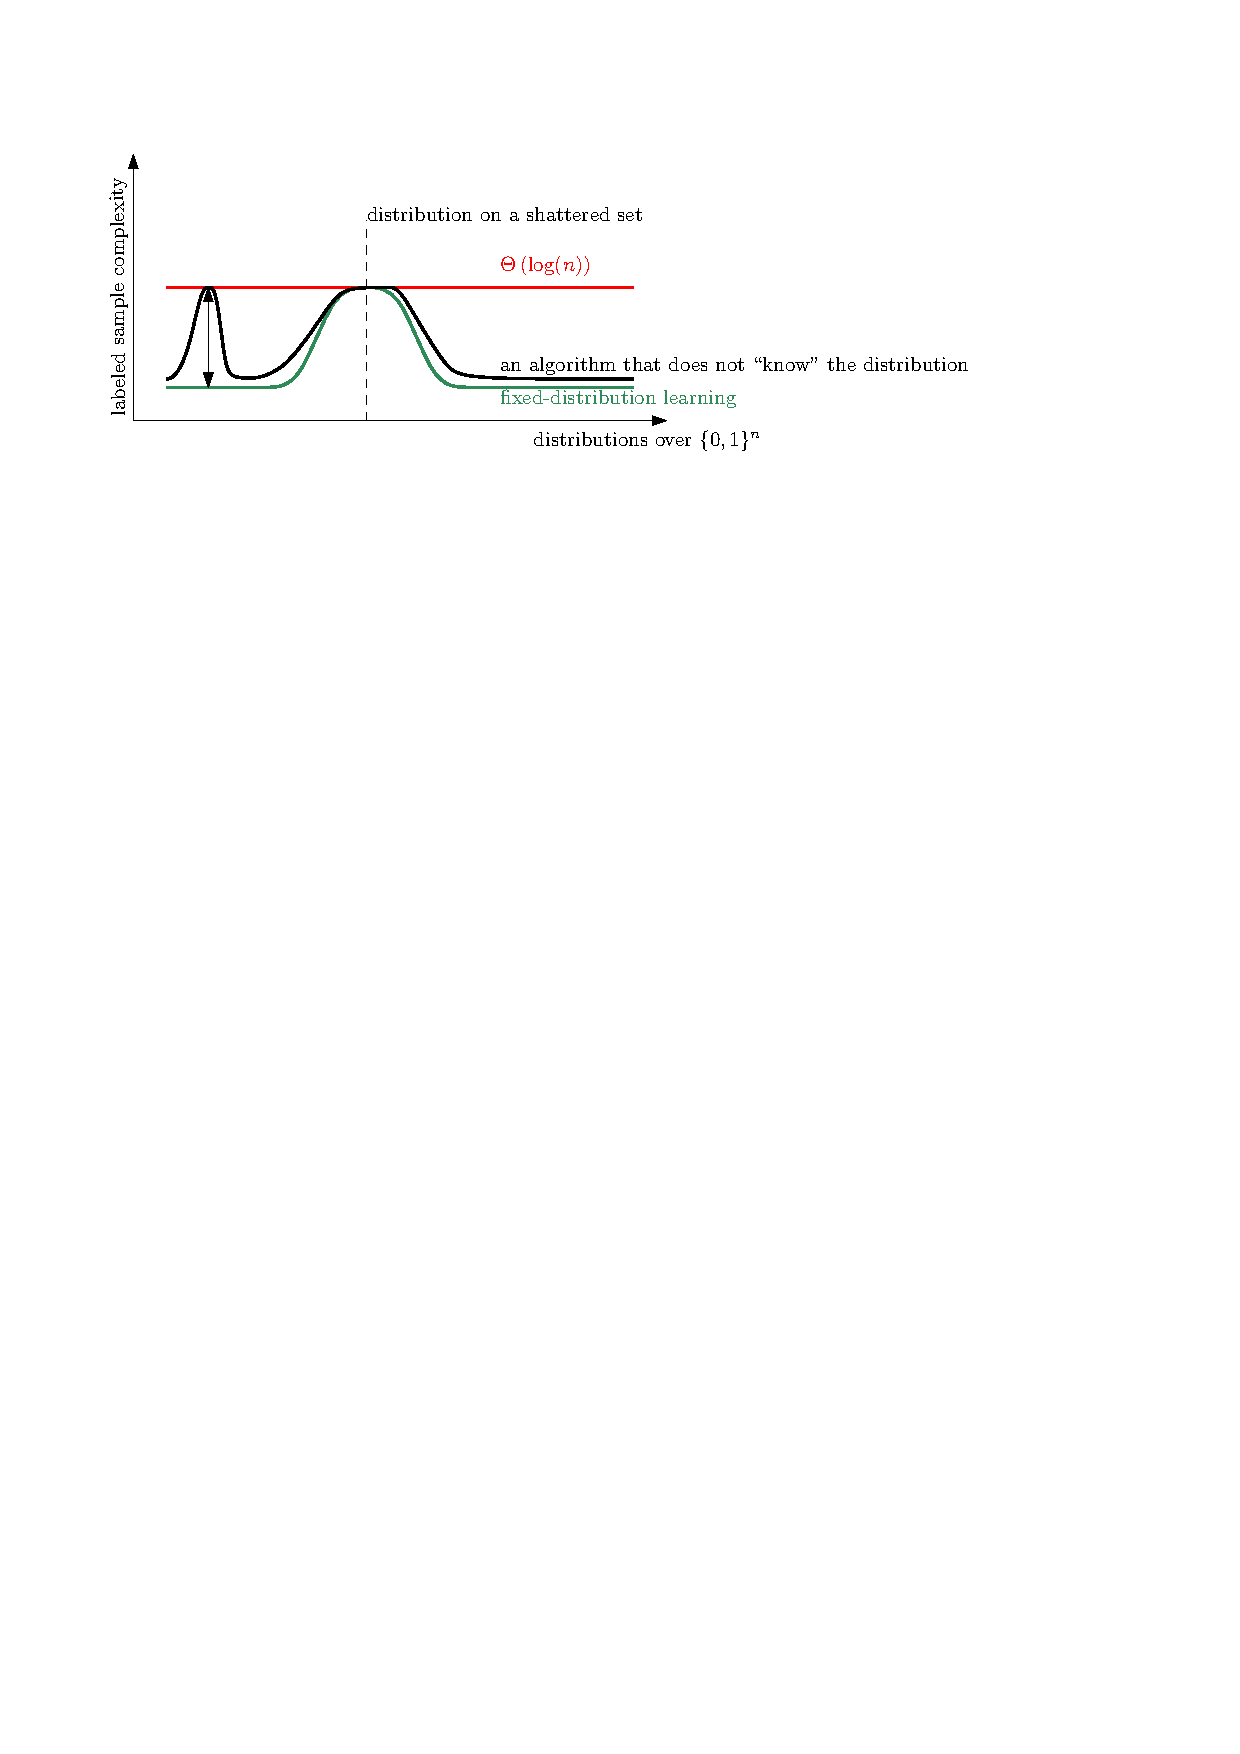
\includegraphics[scale=0.55]{figure}
\caption{\small The graph shows sample complexity bounds of learning a class of
projections over the domain $\{0,1\}^n$ under various unlabeled distributions.
We assume that $\epsilon$ and $\delta$ are constant, say, $\epsilon = \delta =
\frac{1}{100}$. The graph shows three lines. The red horizontal line is
Hanneke's bound for the class of projections, which is $\Theta(\VC(C_n)) =
\Theta(\log n)$. The green line is the Benedek-Itai bound. The green line
touches the red line for certain distributions, but is lower for other
distributions. In particular, for certain distributions the green line is
$O(1)$. The dashed line corresponds to a particular distribution on a shattered
set. This is where the green line and red line touch. Furthermore, here the
upper bound coincides with the lower bound for that particular distribution. The
black line is the sample complexity of an arbitrary
\emph{distribution-independent} algorithm. For example, the reader can think of
the ERM or Hanneke's algorithm. We prove that there exist a distribution where
the black line is $\Omega(\log n)$ times higher than the green line. This
separation is indicated by the double arrow.}
\label{figure:sample-complexity}
\end{figure}

The paper is organized as follows. In \autoref{section:related-work} we review
prior work. \autoref{section:preliminaries} gives the necessary definitions and
basic probabilistic tools. In \autoref{section:projections} we give the proof of
the separation result for projections. In \autoref{section:all-functions} we
prove that there is no gap for the class of all functions. In the full version of the paper, we give a proof of a simple upper bound
$(e/\epsilon)^d$ on the size of the minimum $\epsilon$-cover and a proof of
Benedek-Itai's $O \left( \frac{\log N_{\epsilon/2} + \log
(1/\delta)}{\epsilon}\right)$ sample complexity upper bound.
